\chapter{System Design}\label{chapter:general_design_decisions}

\section{Core Design Decisions}
The Framework is designed to be distributed in nature with the concepts of Actors~[\autoref{sec:actorProgramming}]. It should follow the standard actor programming concept and provide inherently distributed nature to the applications built on top of it. The framework itself should be built using the concept of ‘message-passing’~[\autoref{sec:messagePassing}] to alleviate any possibility of concurrency issues, thus thread-safe.

\begin{itemize}
  \item The framework may not guarantee the delivery of a message.
  \item All the messages sent by the framework will be based on ‘fire and forget’ concept.
  \item A message shall be delivered at most once.
  \item A message should always be routed through Message Queuing System, even though the target isolate may belong to same isolate system in the same logical or physical node.
  \item Feeding of message to an isolate should be based on pull mechanism, not push mechanism.
  \item Exceptions thrown at child isolates shall be handled by a ‘spawnee’ of that isolate. Hence, implementing the idea of supervision and “let it crash” ideology[~\autoref{sec:letItCrash}].
\end{itemize}

\section{The Framework}
\begin{figure}[H]
  \centering
  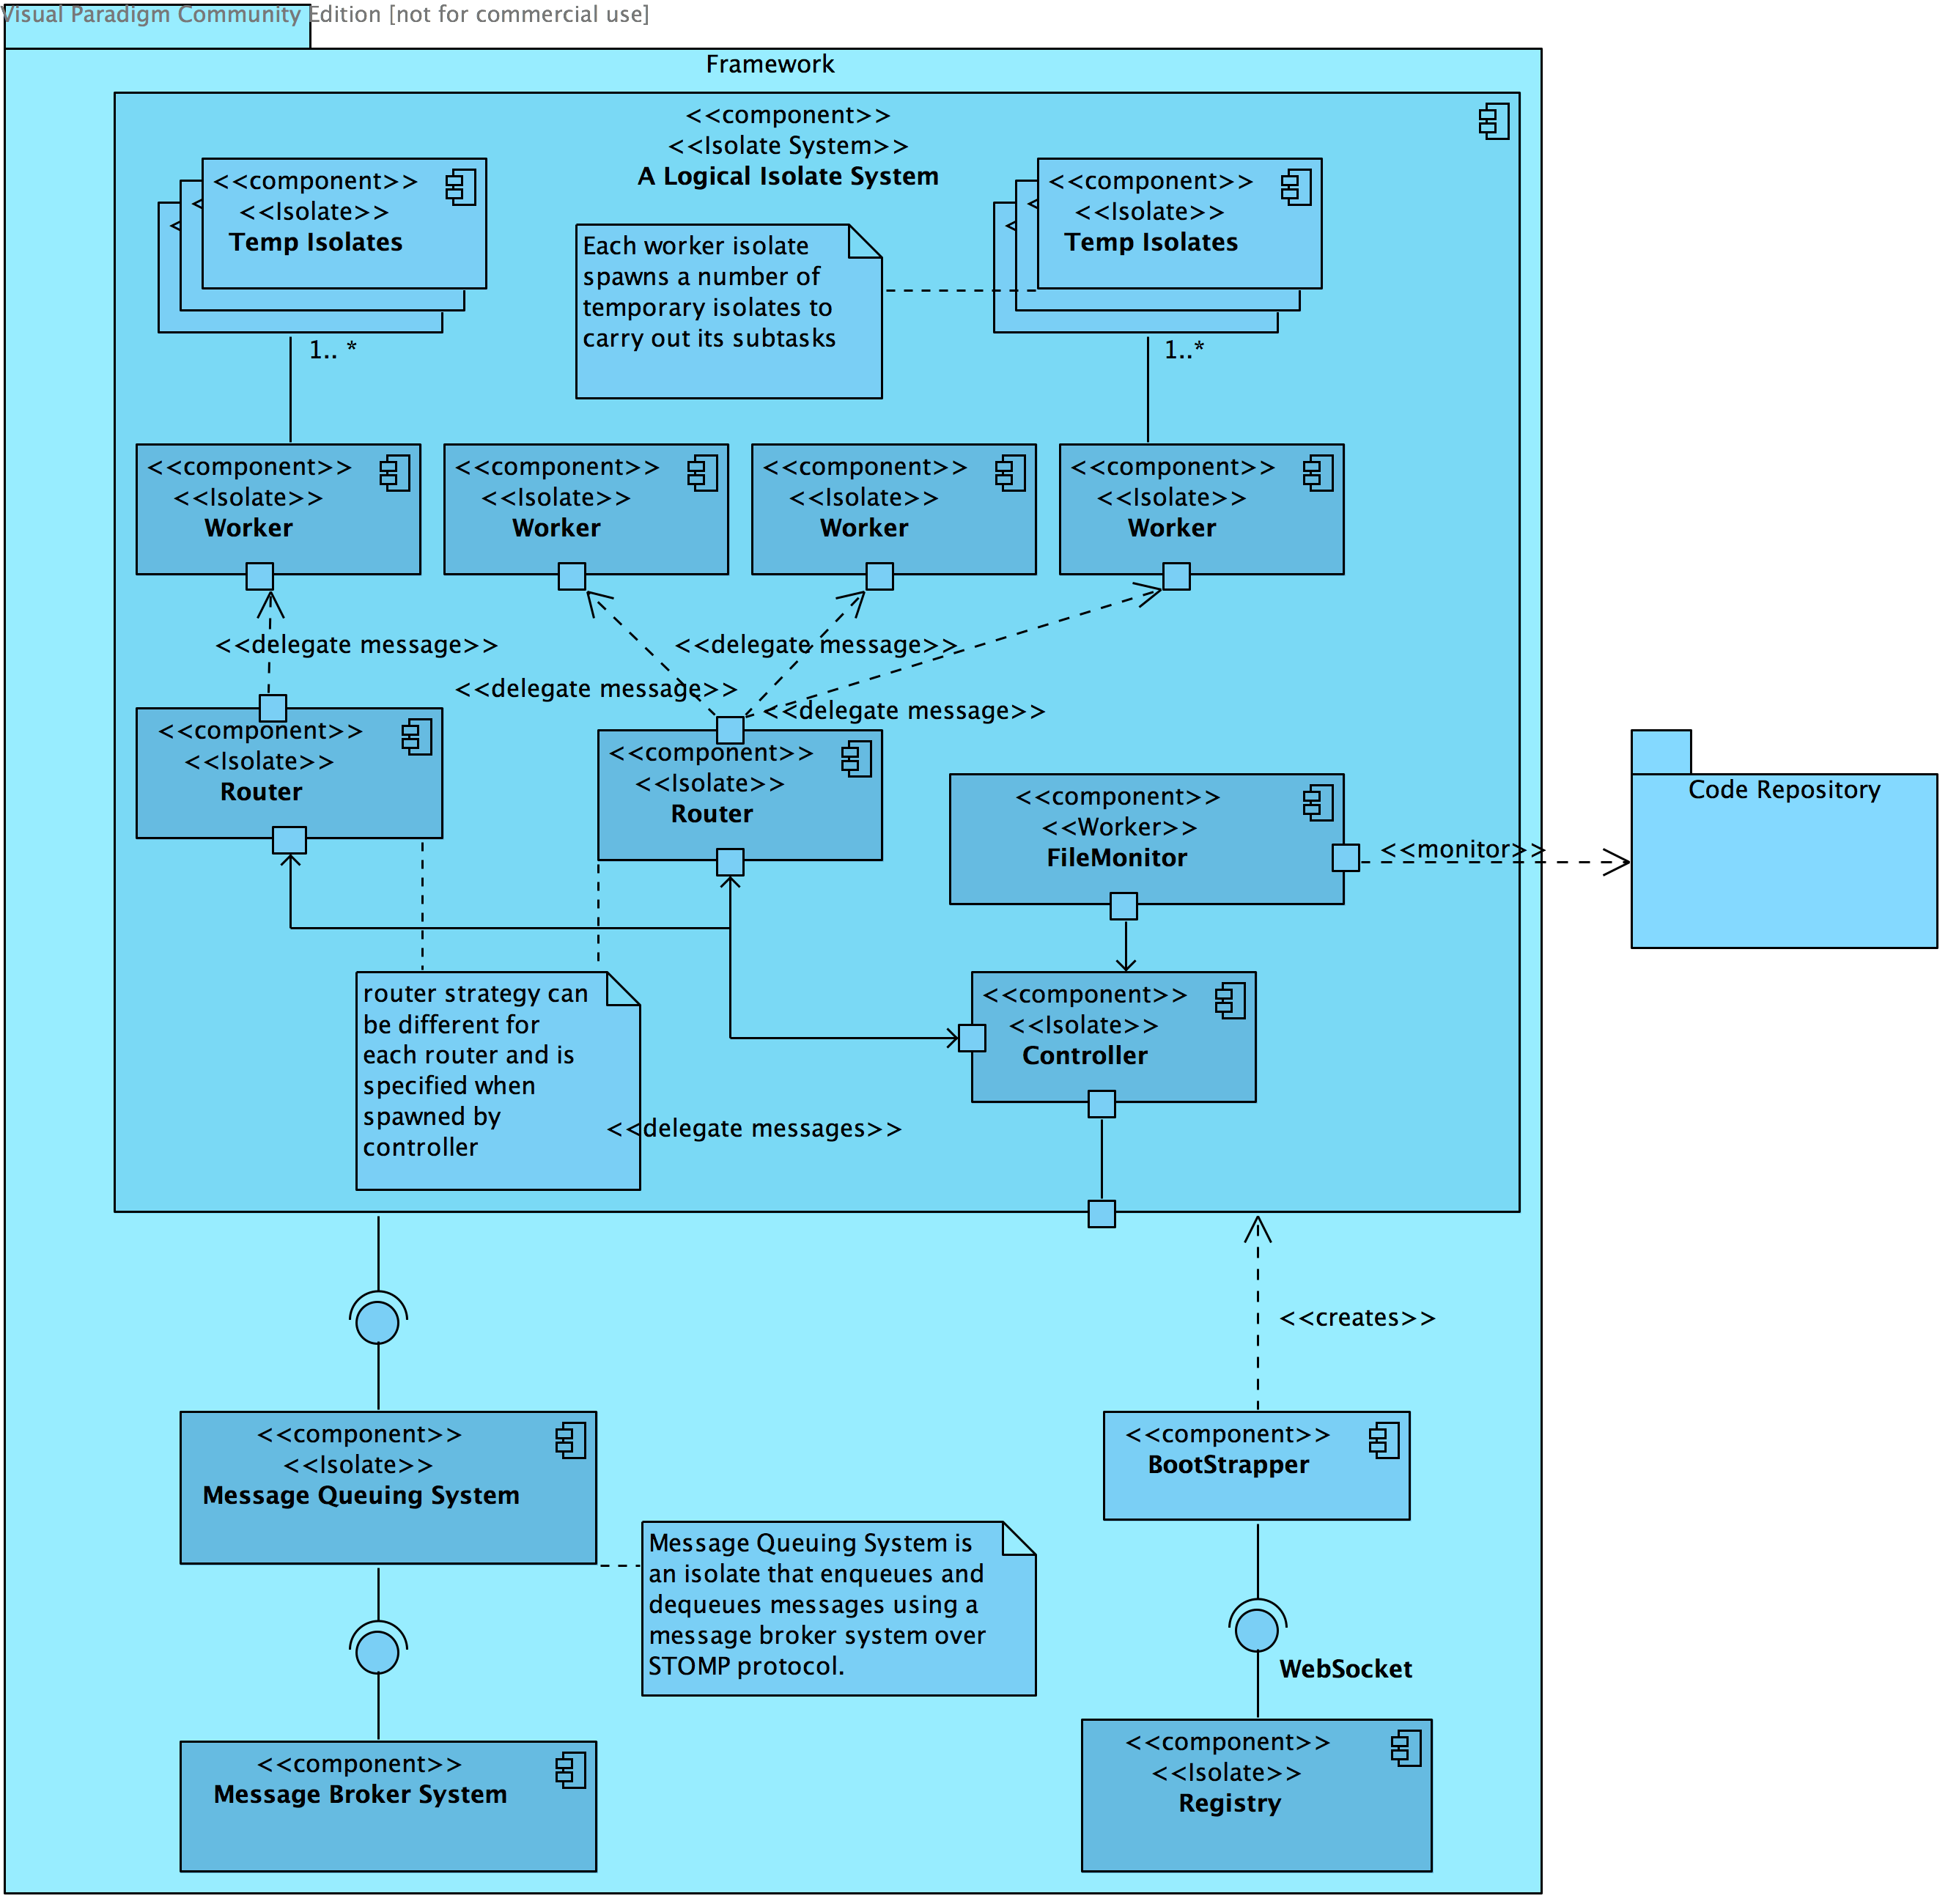
\includegraphics[width=1\textwidth]{figures/componentDiagram}
  \caption[Architecture of the framework]{Architecture of the framework}
  \label{fig:architecture}
\end{figure}


The framework comprises of an Isolate System, a Registry, a Message Queuing System, a Message Broker System and an Activator. The \autoref{fig:architecture} depicts the general overview of different components and sub-components of the framework.

  \subsection{Isolate System}
  An Isolate System is analogous to an actor system. Just as an actor system consists of a group of actors working together, an isolate system is composed of a group of ‘Worker’ isolates working closely. It consists of different hierarchies which forms a logical organizational-like structure. The top level isolate is the Isolate System itself and the bottom most are the ‘Worker’ isolates.

  A ‘Bootstrapper’ in physical node can start up several Isolate Systems. Nevertheless, a logical Isolate System is not limited to a single physical node. The ‘Worker’ isolates spawned by an isolate system can be distributed across several remote systems.

  Each isolate system has its unique id, which is a \acrshort{uuid}. It is generated when the isolate system is bootstrapped. For bootstrapping, an isolate system needs the WebSocket address of Message Queuing System, and a ‘name’ for itself. The name is simply an alias, and should not be confused with the unique id as another isolate system with the same name can exist in other nodes but the unique id is exclusive for a particular instance of an isolate system.

  The bootstrapping of an isolate system includes: generating a new id which is unique for itself, opening up a ‘ReceivePort’, and connecting to a ‘Message Queuing System’. After opening up a ‘ReceivePort’, the isolate system starts listening on that port for messages so that it can receive incoming messages from ‘Controller’. While connecting to the Message Queuing System, if a connectin could not be established, it simply keeps on retrying at certain interval. Furthermore, should the connection be lost at any time after being connected with the MQS, the Isolate System automatically keeps on trying to re-establish the connection at regular interval. Since, the connection to MQS takes place asynchronously, the isolate system simply moves forward and spawns a controller, regardless of the establishment of connection with the MQS.

  \subsubsection{Adding Worker Isolates to The Isolate System}
  As an isolate system is a top level isolate, it spawns a controller. The controller spawns one or several routers and each router spawns a worker isolates. The \autoref{fig:addIsolateSequence} shows the message flow sequence in different components while starting up an isolate system and deploying a worker isolate in it.

  \begin{figure}[H]
    \centering
    \tiny
  \begin{sequencediagram}
  \newinst[0.5]{u}{Developer}
  \newinst[0.5]{reg}{Registry}
  \newinst[0.5]{b}{Bootstrapper}
  \newinst[0.5]{s}{Isolate System}
  \newinst[0.5]{c}{Controller}
  \newinst[0.5]{r}{Router}
  \newinst[0.5]{w}{Worker}

    \mess{b}{connect and register}{reg}
    \mess{u}{deploy isolate}{reg}
    \mess{reg}{initialize isolate system}{b}
    \mess{reg}{add isolate}{b}
    \mess{s}{spawn controller}{c}
    \mess{c}{SendPort}{s}

    \begin{call}{b}{addIsolate()}{s}{}
    \end{call}
    \mess{s}{add isolate}{c}
    \mess{c}{spawn router}{r}
    \mess{r}{SendPort}{c}

    \mess{r}{spawn worker}{w}
    \mess{w}{SendPort}{r}

  \end{sequencediagram}
    \caption{Adding a Worker isolate to an isolate system}
  \end{figure}
  \label{fig:addIsolateSequence}
  \normalsize

  When an isolate system is first initialized, it is an empty system without any Workers running in it. The Workers can be added with appropriate load balancer once the isolate system has been initialized. The ‘addIsolate’ method starts up worker isolates into the isolate system. It requires following arguments:
  \begin{description}
    \item[\itshape{name}] \textendash{} A name for pool of isolates. A deployed isolate has its own name but overall the name is concatenated with the name of isolate system to denote the hierarchy. For instance, an isolate with name ‘account’ becomes ‘bank/account’ where ‘bank’ is the name of the isolate system.
    \item{\itshape{sourceUri}} \textendash{} The location of the source code from which the isolate shall be spawned. The path can either be absolute path to the local file system or the full http or https URI.
    \item{\itshape{workersPaths}} \textendash{} List of destinations where each of the isolates should be spawned. To spawn locally, ‘localhost’ should be used, whereas to spawn in remote node, WebSocket path like: “ws://192.168.2.9:42042/activator” should be used. The number copy of isolates that should be spawned is determined by the length of this list. If multiple copies of isolates should be spawned in a node, the location can be repeated. For instance [“localhost”, “localhost”] results in spawning of two identical isolates in local machine which is load balanced by the type of specified router.
    \item{\itshape{routerType}} \textendash{} The type of load balancing technique that one would like to use to effectively distribute incoming messages. By default, the framework, provides three types of routers: Round-Robin, Random and Broadcast. If the developer wants to use his own customized load balancer instead of using the options provided by the framework, the absolute path to the location of source code, which can also be a remote URI, of the custom router implementation can be provided.
    \item{\itshape{hotDeployment}} \textendash{} This argument is optional and is set to ‘true’ by default. Setting it to ‘true’ enables continuous monitoring of the source code. If any change in source code is identified, the  instances of isolates, spawned by this ‘addIsolate’ function, in current isolate system will be restarted, without the need of redeploying the system.
    \item{\itshape{args}} \textendash{} Custom additional arguments to be passed into each instance of spawned isolate. This argument is also optional and can be safely ignored.
  \end{description}

  \subsubsection{Message Handling in The Top Level Isolate System}
  Typically, a message in an isolate system can arrive from three sources: Message Queuing System via WebSocket, Controller via ReceivePort or Bootstrapper via direct function call. As Dart is a single threaded programming language~[\autoref{sec:isolates}], only one message is handled at a time.

  A Message Queuing System sends the data over WebSocket in JSON string format, which should be deserialized to Map data type before further processing. As the received message contains the queue name from which it is dequeued, the name of the queue is then parsed and transformed to name and address of the corresponding isolate. The message is then forwarded to the Controller that this instance of the isolate system has spawned.

  The messages arriving from Controller is either a dequeue requests or a message that should be sent to the Message Queuing System for enqueuing. The dequeue requests are sent from the isolates that have completed certain task and are ready to accept another message. For the dequeue requests, the sender of the message is identified, which is used to figure out the corresponding name of the queue name. Then the pull request to dequeue from that queue is forwarded to MQS via open WebSocket port. For the messages that are supposed to be delivered to another isolate, the name of the target isolate is used to figure out the name of the queue and then sent to the MQS for enqueuing.

  The ‘Bootstrapper’ of a node that creates an isolate system can send messages to isolate system by directly invoking the functions provided by the isolate system. The bootstrapper can request the information about the isolates this instance of isolate system is running. For which, the isolate system delegates the message to its controller and waits asynchronously for the response from the controller. The request, to fetch a list of running worker isolates, is triggered when a user sends the request to view details of an isolate system via a web interface or via RESTful web service provided by the ‘Registry’~\autoref{subsec:registry}.

  Another type of message is the message to terminate a worker isolate, which is also forwarded to the controller as the isolate system does not directly manage the running worker isolates. Thus, the message is forwarded to the controller which is next in the hierarchy. In contrast, when the shutdown command for the isolate system is triggered via web or REST interface, the isolate system closes all the open ports including WebSocket ports and ReceivePorts, and then wait for the ‘Garbage Collector’ to and clean up the memory reserved by it.

  \subsubsection{Controller}
  Every isolate system has a single controller, which is spawned by the top level isolate of the isolate system. A controller stays idle until it receives a message to create an isolate. Basically, a controller spawns and manages all the routers of an isolate system. Additionally, a controller takes care of the ‘hot deployment’ feature for which it spawns a ‘FileMonitor’ for each router if the feature is enabled. When a RESTART message is received from a FileMonitor, the controller sends a RESTART\textunderscore{}ALL message to the designated router, which restarts all the Worker isolates the router has spawned.

  A controller is also responsible for replying to the query of list of isolates an isolate system is running. It achieves this by keeping a detailed record of each Router and number of Worker isolates each Router is handling, which is updated as soon as an isolate is killed or a new isolate is added.

  As a Controller is the ‘spawner’ of Routers and the ‘spawnee’ of the top level isolate, it forwards the messages as well as dequeue requests coming from Routers to the top level isolate of an isolate system.

  \subsubsection{Router}
  A router is spawned by a controller. The router creates and is responsible for a group of identical Workers isolates. Since an isolate is single threaded, creation of multiple instances of an isolate is desirable for concurrency. When a message arrives in a router from a controller, the router, based on its defined routing policy, delegates the message to one of the worker isolates. The routing policy can be chosen at the time of deployment of a worker isolate.

  A router uses a routing policy to distribute message among the group of isolates it is handling. The default routing policies that are available in the framework are listed in the \autoref{tab:routers}
\begin{table}[htsb]
  \caption[Routing techniques provided by the framework]{List of routing techniques provided by the framework}\label{tab:routers}
  \centering
  \begin{tabular}{l l}
    \toprule
      Router & Description \\
    \midrule
      Round Robin &  Messages are passed in round-robin fashion to its \\ & Worker isolates.\\
      Random &  Randomly picks one of its Worker isolates and sends\\ & the message to that Worker isolate.\\
      Broadcast & Replicates and sends message to all of its Worker isolates.\\
    \bottomrule
  \end{tabular}
\end{table}

    In addition to the available routing policies of the framework, it is also possible to add a new Routing technique by simply extending the ‘Router’ class which requires ‘selectWorker’ function to be implemented. The overridden ‘selectWorker’ function may either return a list of Workers or a single Worker. The ability to implement a custom router opens up possibilities for numerous load balancing techniques. For instance, a simple multicasting router that replicates a message only to the Workers that are spawned locally can be implemented by selecting such Workers using their deployment paths and returning them as a ‘List’.

    As the router manages the Worker isolates it has spawned, it is responsible for effectively terminating and restarting the Worker isolates. It also buffers the messages that might arrive while the workers are not ready to accept the messages yet; usually, during the creation of Worker isolates and while restarting them.

    If a router does not receive any message from a Worker for a certain amount of time, the router sends a PING message to check if the Worker isolate is alive and ready to accept more messages. If the Worker isolate responds with a PONG message, the router sends a request to fetch messages to controller. This mechanism is present in the framework to prevent the ‘starvation’ for a Worker isolate in case the dequeue message, that might have been sent earlier, could not reach the Message Queuing System because of a network issue or unavailability of MQS.

  \subsubsection{Worker}
  The ‘Worker’ of the framework is an abstract class, which should be inherited by the isolate that the programmer creates. The ‘Worker’ first unwraps the messages that arrives from the router and retrieves headers from it. ‘Sender’ and ‘replyTo’ headers of the message is collected before forwarding message to the child class, that extends this abstract class. By unwrapping the messages that is encapsulated by various headers, the abstract Worker class makes sure that the message is delivered to the target implementation of the Worker isolate immutated and in intended form.

  To extend the ‘Worker’ isolate, one must implement ‘onReceive’ function which handles incoming messages and carry out the business logic tasks. However, if a task is too complex, the Worker isolate can divide the tasks into subtasks and spawn temporary isolates to carry out those subtasks concurrently. The temporary isolates can be terminated once the subtask has been carried out.

  The ‘send’, ‘reply’ and ‘ask’ functions are provided by this abstract Worker class to send a message to another worker isolate. These functions automatically add the information of sender and receiver in the header of the message that is sent out.

  \paragraph{Sending a Message}
  \label{para:sendMessage}
  To send a message from one Worker isolate to another, the framework provides ‘send’ function. It takes ‘message’ and ‘address’ of the target Worker isolate as its argument. The reply path can also be optionally set, so that the replied message from target isolate is sent to a different worker isolate for further processing. The named parameter\footnote{Dart's named paramter feature} ‘replyTo’ can be used with the address of actor that is supposed to received the replied message; eg:
\begin{lstlisting}
  send("A simple text message", "demosystem/printer");
  send("Another message", "demosystem/jsonConverter", replyTo: "demosystem/printer");
\end{lstlisting}

  \paragraph{Asking For a Reply}
  \label{subsec:askMessage}
  Sometimes a Worker isolate might need a reply from another isolate for further processing or before replying to the sender of the message. In such case, the worker isolate can specifically ask the target isolate to reply to this particular instance of worker isolate.

  For instance, a sample use case can be, a worker isolate maintaining a connection with a browser via HTTP. In this case, as the port cannot be serialized and passed to other isolates through messages, another instance of similar isolate will not be able to respond to the request made in that connection.

  Similar to the ‘send’ function, the ‘ask’ function takes ‘message’ and ‘address’ of the target worker isolate as its argument; eg:
\begin{lstlisting}
  ask("current time", "demosystem/timeKeeper");
\end{lstlisting}
  \paragraph{Replying to a Message}
  \label{subsec:replyMessage}

  To reply to a message, the framework provides the ‘reply’ function. It expects a single argument~\textemdash{} ‘message’, because the respose is sent to the worker isolate specified by the sender. The ‘reply’ can be used in response to any of ‘send’ or ‘ask’ messages; eg:
\begin{lstlisting}
  reply("Current time is: $time");
\end{lstlisting}

  \subsubsection{Proxy}
  A ‘Proxy’ is the special type of a Worker isolate. When a Worker isolate is supposed to be spawned in a remote node, the router instead spawns a Proxy isolate in local node. Once the Proxy isolate is created, it connects to the ‘Isolate Deployer’ of the remote node where the Worker isolate is intended to be spawned. After establishing connection over a WebSocket with Isolate Deployer of the remote node, the proxy isolate forwards the request to spawn the worker isolate to the Isolate Deployer. After successful spawning of isolate in the remote node, the proxy isolate simply forward the messages that is sent to it by the spawner router. Each proxy worker maintains a separate WebSocket connection with an ‘Isolate Deployer’.\\

  \begin{figure}[H]
    \centering
    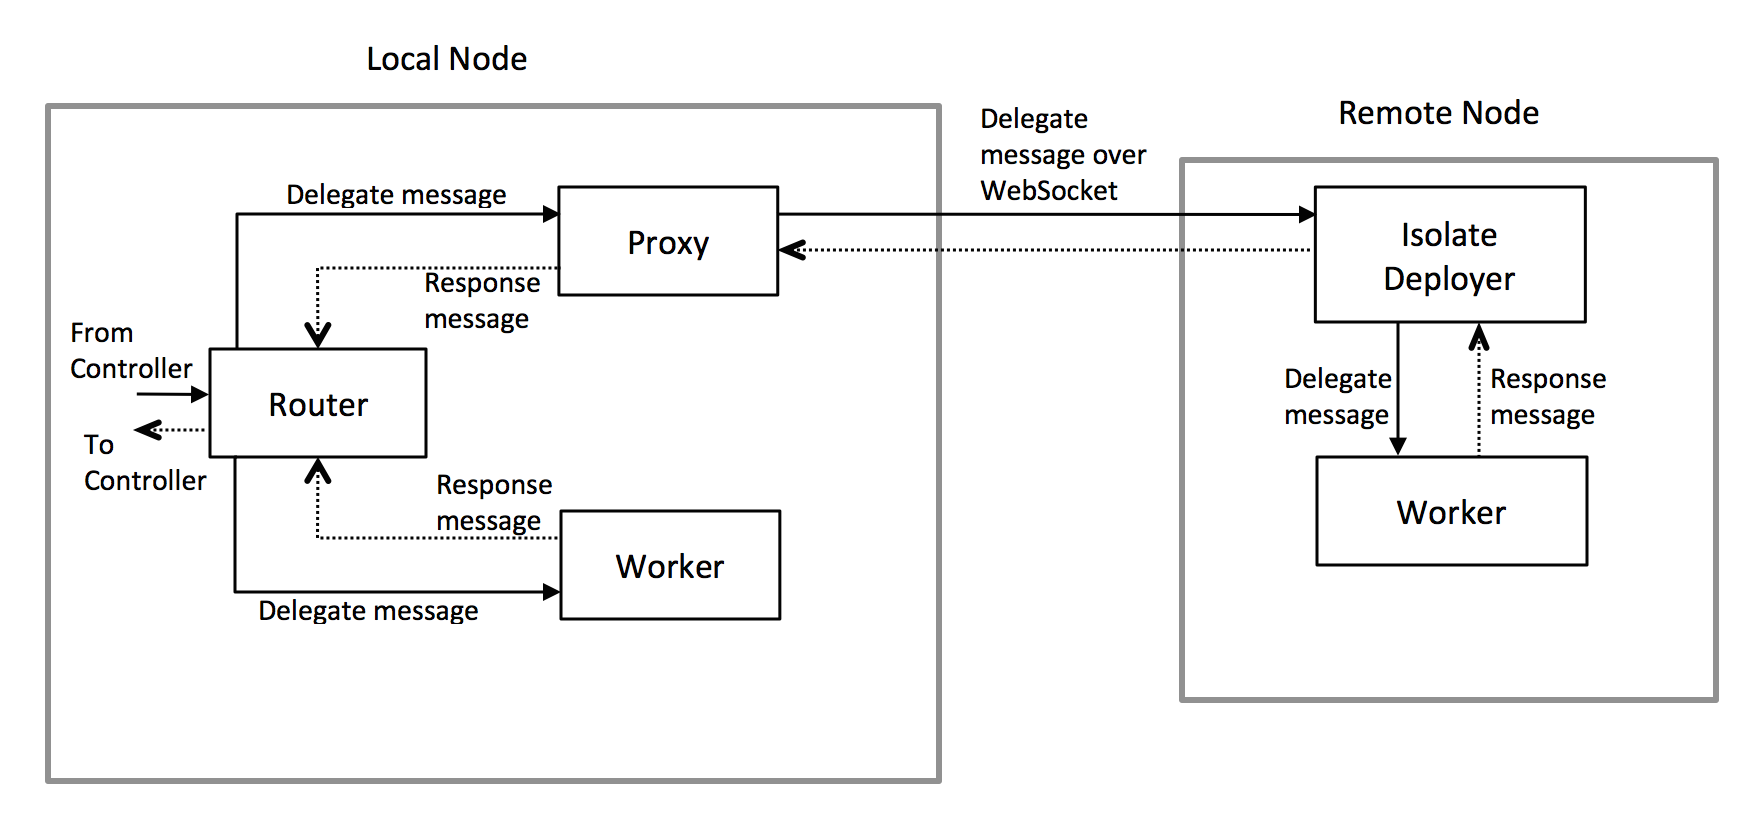
\includegraphics[width=1\textwidth]{figures/proxy}
    \caption[Proxy Worker]{A Proxy Worker}
    \label{fig:proxy}
  \end{figure}

  \subsubsection{FileMonitor}
  \label{subsubsec:fileMonitor}
  The controller spawns a ‘FileMonitor’ only if the ‘Hot Deployement’ flag for an worker isolate is set while deploying. The spawned ‘FileMonitor’ monitors the md5 checksum of the source code using which the Worker isolate is spawned. If a change in the source file is detected, it simply sends a RESTART command to the controller, which eventually forwards it to the target router. The router then restarts all of its worker isolates.

\subsection{The Registry}
\label{subsec:registry}
The Isolate Registry is a central node where other nodes, which are running Bootstrapper, connect and register themselves. The registry simply keeps the record of the connected nodes, assigns a unique id to each and queries them about the running isolate systems when required. The registry provides RESTful API and a web interface~\footnote{the web interface can be opted out as it has to be started separately} through which one can have an overview of the full system and manage the deployments of the isolate systems as well as individual isolates.

The basic tasks that a registry carries out are:
\begin{itemize}
  \item Bootstraps an isolate system, during runtime, in local or remote node
  \item Provides a way to deploy, update or remove an isolate system
  \item Returns information about the deployed isolates by querying the individual isolate system of a node.
\end{itemize}

  \subsubsection{RESTful API of Registry}
  \label{subsec:restApi}
  The registry provides a REST API to perform the operations on the connected nodes. One can send a ‘GET’ request to the registry to fetch the list of the nodes that are connected to the registry. Using the ‘id’ of a node from the replied list, one can deploy an isolate system or add an isolate to already deployed system by sending appropriate ‘POST’ request.

  The REST endpoints exposed by the registry are listed in table~\autoref{tab:endpoints}.
  \begin{table}[htsb]
    \caption[Endpoints exposed by the registry]{List of endpoints exposed by the registry}\label{tab:endpoints}
    \centering
    \begin{tabular}{l l}
      \toprule
        Method  & Endpoint \\
      \midrule
        GET &  /registry/system/list\\
        GET & /registry/system/\{bootstrapperId\} \\
        POST & /registry/deploy \\
        POST & /registry/system/shutdown \\
      \bottomrule
    \end{tabular}
  \end{table}

\paragraph{A sample GET and POST query to deploy an isolate system}
\begin{description}
  \item{GET request to fetch a list of connected systems}\\
  Request: ‘GET \url{http://54.77.239.254:8000/registry/system/list}’\\
  Response Status Code: 200 OK\\
  Response Body:
  \begin{lstlisting}[language=json,firstnumber=1]
    [
      {
        "bootstrapperId": "266393094",
        "ip": "54.77.239.244",
        "port": "50189"
      },
      {
        "bootstrapperId": "12133208",
        "ip": "54.77.239.243",
        "port": "50192"
      }
    ]
  \end{lstlisting}

  \item{POST request to deploy an isolate system}\\
  Request: ‘POST \url{http://54.77.239.254:8000/registry/deploy}’\\
  Request Body:
  \begin{lstlisting}[language=json,firstnumber=1]
    {
      "bootstrapperId" : "266393094",
      "action": "action.addIsolate",
      "messageQueuingSystemServer": "ws://54.77.239.200:42043/mqs",
      "isolateSystemName" : "sampleSystem",
      "isolateName" : "consumer",
      "uri" : "http://54.77.239.221/sampleSystem/bin/Consumer.dart",
      "workersPaths" : ["localhost", "ws://54.77.239.243:42042/activator"],
      "routerType" : "random",
      "hotDeployment" : true
    }
  \end{lstlisting}
  Response Status Code: 200 OK
\end{description}

\paragraph{A sample GET query to fetch details of an isolate system}
  \begin{description}
    \item{GET request to get details of an isolate system}\\
    Request: ‘GET \url{http://54.77.239.254:8000/registry/system/266393094}’\\
    Response Status Code: 200 OK\\
    Response Body:
    \begin{lstlisting}[language=json,firstnumber=1]
    {
      "sampleSystem": [
        {
          "id": "sampleSystem/consumer",
          "workerUri": "http://54.77.239.221/sampleSystem/bin/Consumer.dart",
          "workersCount": 2,
          "workersPaths": [
            "localhost",
            ws://54.77.239.243:42042/activator"
          ],
          "routerType": "random",
          "hotDeployment": true
        }
      ]
    }
  \end{lstlisting}
  \end{description}

\paragraph{A sample POST query to terminate a Worker isolate}
  \begin{description}
    \item{POST request to terminate an isolate of an isolate system}\\
    Request: ‘POST \url{http://54.77.239.254:8000/registry/system/shutdown}’\\
    Request Body:
    \begin{lstlisting}[language=json,firstnumber=1]
      {
        "bootstrapperId" : "266393094",
        "isolateSystemName" : "sampleSystem",
        "isolateName" : "consumer"
      }
    \end{lstlisting}
    Response Status Code: 200 OK
  \end{description}

\paragraph{An example of terminating an Isolate System}
  \begin{description}
    \item{POST request to terminate an isolate of an isolate system}\\
    Request: ‘POST \url{http://54.77.239.254:8000/registry/system/shutdown}’\\
    Request Body:
    \begin{lstlisting}[language=json,firstnumber=1]
      {
        "bootstrapperId" : "266393094",
        "isolateSystemName" : "sampleSystem"
      }
    \end{lstlisting}
    Response Status Code: 200 OK
  \end{description}

The registry generates all the information about isolate and isolate systems “on the fly”. Thus, it does not need to persist any data.

  \subsubsection{The Web Interface for the Registry}
  The deployment of isolates can also be managed by using a web interface provided by the registry. The Web Interface should be started up separately in a different port. The Web Interface, internally communicates with the registry via the REST API~[\ref{subsec:restApi}] which is exposed by the Registry.

  <TODO: A Screenshot here or in the Appendix>

\subsection{Message Queuing System (MQS)}
  Since, the basis of this system is message passing, the Message Queuing System is an important component of this framework. The MQS is a top level isolate that fetches messages from message broker system and dispatches to respective isolate of the isolate system. Whenever a new isolate system starts up, it opens up a new WebSocket connection with the MQS. The messages are exchanged between the isolate system and the MQS through the WebSocket connection. The MQS keeps track of the unique-id of an isolate system so that it can identify the origin of the message.

  If a message is supposed to be enqueued, the MQS ignores the unique-id and simply forwards the message to the ‘Enqueuer’ isolate. Whereas, if the message is a dequeue request, the MQS forwards the the message to a ‘Dequeuer’ isolate along with the unique-id of the isolate system. The unique-id is used to identify the WebSocket port through which the request arrived. Thus, making sure that the dequeued message is sent to the correct requester. This is especially required if a cluster, of identical isolate systems, is running on different nodes.

  The MQS should be started up separately along with few command line arguments to connect to message broker system. The required command line arguments are: ip address, port, username and password to connect to Message Broker System. The ‘prefetchCount’ is an optional argument which defaults to 1, if not provided explicitly. A ‘prefetchCount’ is a Quality of Service header for Message Broker System which allows a subscriber of a queue to hold the defined quantity of unacknowledged messages.

Since, in Dart\footnote{Dart version 1.7.2} the passing of sockets to isolates is not yet possible, so the main isolate has to pipe all the input/output data. In this case the MQS is the top level isolate which has to handle all incoming and outgoing messages.

  \subsubsection{Enqueuer}
  An enqueuer is a separate isolate. A Message Queuing System has only one enqueuer, which basically receives messages from the MQS and sends messages to a message broker system \textendash{} RabbitMQ~[\ref{sec:rabbitmq}] via STOMP~[\ref{sec:stomp}] protocol.

  \subsubsection{Dequeuer}
  As opposed to Enqueuer, a Message Queuing System maintains each dequeuer for each topic. The topic corresponds to each router running in the isolate system. Whenever a message arrives from a new isolate, the MQS spawns a new dequeuer isolate. The dequeuer then subscribes to a new message queue in the message broker system via STOMP~[\ref{sec:stomp}] protocol. If the queue does not exist in the message broker system, the message broker system automatically creates the queue.

  If a dequeuer is idle for too long, i.e. if the Dequeuer isolate has not received any dequeue requests for certain interval\footnote{by default the timeout is 10 seconds}, then the MQS terminates the dequeuer isolate for that particular queue. Nevertheless, as soon as the MQS receives a dequeue request, it spawns a new Dequeuer, if one does not exist yet.

  The dequeuer subscribes messages from Message Broker System with such options that the new messages do not arrive to the subscriber unless previously dequeued messages have been acknowledged. This throttles the flow of messages from message broker system and keeps itself and the isolates from being overwhelmed by large number of messages, which might induce ‘out of memory’ issues.

  Messages in dequeuer keeps on arriving as long as there are messages in the queue and the messages are being acknowledged. The messages that are in the buffer of dequeuer stay in unacknowledged state unless they are flushed and sent out to the requesting isolate of an isolate system. As soon as a message is acknowledged the dequeuer receives another message from the message broker.

  \subsubsection{Multiple Instances of MQS}
  It is possible for a system to have multiple Message Queuing Systems for scaling up the system. If there are multiple identical isolate systems connected to different instances of MQS, each MQS will have a dequeuer which subscribes to the same queue. Nevertheless, a message is dispatched by the message broker system to only one of the dequeuers, which is distributed in round robin fashion. Thus, messages are fairly distributed among the subscribers.

\subsection{Activator}
  An activator simply starts up two isolates: a ‘System Bootstrapper’ and an ‘Isolate Deployer’. Every node that is supposed to be running an Isolate System or become a part of isolate system by running isolates must be running an Activator. The activator requires a WebSocket address of the Registry as a command line argument. Nevertheless, it is also possible to start up System Bootstrapper and Isolate Deployer separately.

  \subsubsection{System Bootstrapper}
  The System Bootstrapper registers itself to the ‘Registry’ via a WebSocket connection as soon as it is started. The activator forwards the path of the WebSocket to the system bootstrapper. But, if a System Bootstrapper is started separately then the path of the Registry should be passed as a command line argument.

  \subsubsection{Isolate Deployer}
An Isolate Deployer starts up a Worker isolate in a node. The isolate is spawned without a local isolate system and as a part of an isolate system running in another node. This functionality expands the isolate system beyond a physical system. An isolate system can deploy number of instances of an isolate in several different nodes.

  An isolate deployer running in a remote machine is able to handle requests from multiple ‘Proxies’ from several isolate systems. Each proxy opens up a separate WebSocket channel with the isolate deployer.

\section{Some Key Features}
\subsection{Hot Deployment of Isolates and Isolate Systems}
It is possible for the source code, of an isolate, to reside in a remote repository and fetched by the controller of a node when required. For instance: isolate source code can reside in a git repository hosted in GitHub. So that as soon as new code is committed in the repository, it gets immediately picked up by the application and the change gets reflected without restarting the application.

  After a node is bootstrapped, changes like: addition, update or removal of isolates in an isolate system can take place. In such case, the isolates can be killed and redeployed when it has finished processing tasks and is sitting idle. A dedicated isolate ‘FileMonitor’~[\autoref{subsubsec:fileMonitor}] monitors changes in the code repository. When a change is detected, the ‘FileMonitor’ isolate sends a RESTART message along with the target router to notify the controller. The controller takes care of pushing the message to relevant router, and the router takes care of terminating and re-spawning the worker isolates.

  This hot deployment capability improves the availability of an application. Whenever there is any change in a component of an application, the whole application does not need to be re-deployed, instead, only a set of isolates that should be updated is restarted at runtime. This increases overall up-time of the application and keeps other components working even in the time of modifications.

\subsection{Migration of Isolates and Isolate Systems}
  Relocation of Worker isolates or an isolate system during runtime i.e. killing a set of Worker isolates or an isolate system at one node and bringing up same set of Worker isolates in another node is the migration of isolates or isolate system. The concept of hot deployment and migration brings enormous possibilities in a distributed system. Some of them are:

\begin{itemize}

  \item Migration of actors/isolates allows an application to scale in an easy way. With this capability, it is also possible for an application to be brought up the most frequently used isolates near to the server where it is accessed the most.

  \item Related and dependent isolates can be migrated to the same server, if it is evident that it improves performance of the entire system.

  \item In case of hardware failure on a system which is running a certain set of isolates, migration of worker isolates during runtime can make the application survive the hardware failure.

\end{itemize}

\subsection{Remote Isolates}
\label{subsec:remoteIsolate}
  The current isolate implementation in Dart\footnote{Dart version 1.7.2} cannot communicate with other isolates over a network. The Worker isolates in this framework have an ability to communicate with the isolates that may be running in a remote node. So, there can be isolates running in any node. The communication underneath is taken care of by the framework so the implementer of this framework does not have to worry if an isolate is remotely spawned or locally spawned.

  Two isolates, although, running in two different virtual machines, can still belong to a same logical isolate system.

\section{Typical Message Flow in the System}
The framework is based on ‘fire-and-forget’ principle of message sending. The \autoref{fig:enqueueMessage} shows a simple message flow while enqueuing a message and the \autoref{fig:dequeueMessage} shows the process of dequeuing a message.
A message is serialized to JSON string before sending via a SendPort of an isolate and deserialized after receiving from ReceivePort.

\begin{figure}[H]
  \centering
  \tiny
\begin{sequencediagram}
\newinst[0.5]{w}{Worker (Entry point)}
\newinst[0.5]{r}{Router}
\newinst[0.5]{c}{Controller}
\newinst[0.5]{s}{Isolate System}
\newinst[0.5]{m}{MQS}
\newinst[0.5]{e}{Enqueuer}
\newinst[0.5]{rab}{RabbitMQ}

  % \mess{u}{send message}{w}
  \mess{w}{serialize and send message}{r}
  \mess{r}{delegate message}{c}
  \mess{c}{delegate message}{s}
  \mess{s}{delegate message}{m}
  \mess{m}{delegate message}{e}
  \mess{e}{enqueue message}{rab}

\end{sequencediagram}
  \caption{Enqueuing a message}
  \label{fig:enqueueMessage}
\end{figure}
\normalsize

\begin{figure}[H]
  \centering
  \tiny
\begin{sequencediagram}
\newinst[0.5]{w}{Idle Worker}
\newinst[0.5]{r}{Router}
\newinst[0.5]{c}{Controller}
\newinst[0.5]{s}{Isolate System}
\newinst[0.5]{m}{MQS}
\newinst[0.5]{deq}{Dequeuer}
\newinst[0.5]{rab}{RabbitMQ}

  \mess{w}{done}{r}
  \mess{r}{dequeue request}{c}
  \mess{c}{dequeue request}{s}
  \mess{s}{dequeue request}{m}
  \mess{m}{dequeue request}{deq}
  \mess{deq}{acknowledge buffered messages}{rab}
  \mess{deq}{flush buffered messages}{m}
  \mess{rab}{new messages}{deq}
  \mess{m}{dequeued messages}{s}
  \mess{s}{dequeued messages}{c}
  \mess{c}{dequeued messages}{r}
  \mess{r}{route dequeued messages}{w}
\end{sequencediagram}
  \caption{Dequeuing a message}
  \label{fig:dequeueMessage}
\end{figure}
\normalsize

\subsection{Sample message formats}

\subsubsection{The message sent through different components while enqueuing}

\begin{description}

\item Original Message:
\begin{lstlisting}[language=json,numbers=none]
"Test"
\end{lstlisting}

\item Worker:
\begin{lstlisting}[language=json,numbers=none]
{senderType: senderType.worker, id: sampleSystem/producer/88f52440-5060-11e4-f396-97cebb949945, action: action.send, payload: {sender: sampleSystem/producer, to: sampleSystem/consumer, message: Test, replyTo: null}}
\end{lstlisting}

\item Router:
\begin{lstlisting}[language=json,numbers=none]
{senderType: senderType.router, id: sampleSystem/producer, action: action.send, payload: {sender: sampleSystem/producer, to: sampleSystem/consumer, message: Test, replyTo: null\}\}
\end{lstlisting}

\item Controller:
\begin{lstlisting}[language=json,numbers=none]
{senderType: senderType.controller, id: sampleSystem/producer, action: action.send, payload: {sender: sampleSystem/producer, to: sampleSystem/consumer, message: Test, replyTo: null\}\}
\end{lstlisting}

\item Top level isolate:
\begin{lstlisting}[language=json,numbers=none]
{targetQueue: sampleSystem.consumer, action: action.enqueue, payload: {sender: sampleSystem/producer, message: Test, replyTo: null}}
\end{lstlisting}

\item Message Queuing System:
\begin{lstlisting}[language=json,numbers=none]
{topic: sampleSystem.consumer, action: action.enqueue, payload: {sender: sampleSystem/producer, message: Test, replyTo: null}}
\end{lstlisting}

\item Enqueuer:
\begin{lstlisting}[language=json,numbers=none]
  {sender: sampleSystem/producer, message: Test, replyTo: null}
\end{lstlisting}
\end{description}

\subsubsection{Sample format of a message sent at different components while dequeuing}
\begin{description}
\item Dequeuer:
\begin{lstlisting}[language=json,numbers=none]
{"sender":"mysystem/producer","message":"Test","replyTo":null}
\end{lstlisting}

\item Message Queuing System:
\begin{lstlisting}[language=json,numbers=none]
{senderType: senderType.dequeuer, topic: mysystem.consumer, payload: {sender: mysystem/producer, message: Test, replyTo: null}
\end{lstlisting}

\item Top level isolate of isolate system:
\begin{lstlisting}[language=json,numbers=none]
{senderType: senderType.isolate_system, id: mysystem, action: action.none, payload: {to: mysystem/consumer, message: {sender: mysystem/producer, message: Test, replyTo: null}}}
\end{lstlisting}

\item Controller:
\begin{lstlisting}[language=json,numbers=none]
{senderType: senderType.controller, id: controller, action: action.none, payload: {to: mysystem/consumer, message: {sender: mysystem/producer, message: Test, replyTo: null}}}
\end{lstlisting}

\item Router:
\begin{lstlisting}[language=json,numbers=none]
{senderType: senderType.router, id: mysystem/consumer, action: action.none, payload: {sender: mysystem/producer, message: Test, replyTo: null}}
\end{lstlisting}

\item Worker:
\begin{lstlisting}[language=json,numbers=none]
"Test"
\end{lstlisting}

\end{description}

\subsection{Some Implementation Overview}
  Some insight about the implementation of selected functions of the framework:

  \begin{description}
    \item How ‘send’ works?\\
      When a Worker Isolate sends a message using ‘send’ function of the Worker class, the message is encapsulated with further information about the sender and the receiver are added to the message. The encapsulated message is forwarded to the spawner isolate, which in this case, is the router. The router agains forwards it to the controller which again forwards to the top level isolate. Then the top level isolate adds another level of encapsulation and headers to the message so that the Message Queuing System knows the destination queue.

      If the Worker isolate is expecting to consume another message after sending a message, it should send a PULL Request for another message, which can be performed by invoking the ‘done’ function.

      \item How ‘ask’ works?\\
    Ask function has certain subtle differences from the ‘send’ function. The ‘ask’ function should be used when the sender of the message expects something in reply. The abstract Worker class adds the full path of the isolate along with the unique-id of the isolate when an ‘ask’ message is constructed. This is to make sure that the response from the target isolate reaches this particular instance of the isolate. The Router, which can also be called a load balancer, when receives a message with full address of a Worker isolate, routes the message to the isolate with the unique-id contained in the message. The message is simply discarded by the Router, if the isolate with the given unique-id is not found in the list of isolates the Router is maintaining. This is possible when the isolates have been restarted or for some reason the isolate was killed.

    \item How ‘reply’ works?\\
    The ‘reply’ function is simply a convenience for the implementer. The ‘reply’ function simply invokes ‘send’ message with the sender’s address as the target isolate. If the message contains ‘replyTo’ then the message will be replied to the address contained in ‘replyTo’ instead of the original sender. The ‘reply’ function can be used to reply message in both \textendash{} ‘send’ and ‘ask’ cases.

    \item How ‘KILL’ works?\\
    This is a special control message sent to the isolates as well as isolate system to shutdown themselves. If a KILL message is sent to a Worker isolate, the message is enqueued to the end of the Worker isolate as any other message. No further messages after KILL a message are sent to that isolate by the router. The router then buffers the messages until the isolate is restarted and resumes sending messages again once the Worker isolate is spawned.

    When a Worker isolate finishes processing queued messages and encounters the KILL message, the isolate closes its ReceivePort\footnote{A Worker Isolate receives message from Router via a ReceivePort} and stays idle. After sometime it gets ‘Garbage Collected’ and is cleaned up. But, sometimes the garbage collector cannot clean up the isolate and the memory leak occurs. Thus, as a workaround for this, a custom Exception is thrown deliberately by the isolate to terminate itself. The exception is thrown only after it closes all the ports. This workaround forcefully terminates the isolate and releases the memory occupied by the isolate.

    The framework provides \emph{beforeKill()} method, which can be overridden to perform custom operations before terminating an isolate.

    \item How RESTART works?\\
    Restarting an isolate is basically a combined process of killing an isolate and spawning it up again. However, during the restart, after issuing the KILL message, the messages may keep coming from the controller to the router. These messages are buffered in the router itself. The buffered messages are flushed and sent out once the Worker isolates are spawned. For instance, when the ‘Hot Deployment’\autoref{subsec:hotDeployment} feature is enabled, if the source code of the isolate is modified and saved, the each of the isolates that the router has spawned gets restarted. During which the messages that arrive after RESTART message are buffered in the router.

    \item How shutting down an isolate system works?\\
    An isolate system that is running in a node can be shutdown via the Web Interface or via POST request to the registry. When a request to shutdown an isolate system is sent, the isolate system closes all the ports including the isolate ports as well as the WebSocket connection with Message Queuing System. After that the forceful shutdown is carried out by throwing out a custom Exception. This is a work-around to free up the memory consumed after it is shutdown, because the feature to immediately terminate an isolate is yet to be implemented in dart.
  \end{description}

\subsection{Clustering}
  Clustering can be achieved in the framework in several levels.
  \begin{itemize}
  \item By deploying worker isolates in several remote nodes. i.e. taking advantage of the concept of ‘Remote Isolates’~[\autoref{subsec:remoteIsolate}].
  \item By deploying replicas of an isolate system in different nodes. An isolate system with same name can exist in another node even though they connect to the same MQS.
  \item The Message Queuing System itself, can also be replicated where replicas of isolate system may connect to different instance MQS.
  \item Since, several instances of RabbitMQ~[\autoref{sec:rabbitmq}] can form a logical group, sharing common configuration, properties, users, queues etc., a cluster of message broker system can be formed. Which allows, Message Queuing Systems to connect to the different member of a cluster.
  \end{itemize}
<TODO: a simple diagram>
\section{Dart Libraries Used in Construction}
\begin{table}[htsb]
  \caption[Dependent libraries of the framework]{List of libraries directly used by the framework}\label{tab:libraries}
  \centering
  \begin{tabular}{l l}
    \toprule
      Library & URL \\
    \midrule
      path &  \url{https://pub.dartlang.org/packages/path}\\
      uuid &  \url{https://pub.dartlang.org/packages/uuid}\\
      crypto &  \url{https://pub.dartlang.org/packages/crypto}\\
      stomp &  \url{https://pub.dartlang.org/packages/stomp}\\
    \bottomrule
  \end{tabular}
\end{table}

\section{A Sample Implementation of Worker Using The Framework}
\begin{lstlisting}[language=java,firstnumber=1]
    import 'dart:isolate';
    import 'package:isolatesystem/worker/Worker.dart';

    main(List<String> args, SendPort sendPort) {
      Consumer printerIsolate = new Consumer(args, sendPort);
    }

    class Consumer extends Worker {
      Consumer(List<String> args, SendPort sendPort) : super(args, sendPort);

      @override
      onReceive(message) {
        switch(message['action']) {
          case "print":
            print("message['content']");
            break;
          case "send_back":
            reply(message['content']);
            break;
        }
        done();
      }
    }

\end{lstlisting}
